\documentclass[tikz, border=1mm]{standalone}

\begin{document}
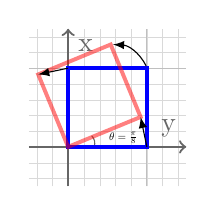
\begin{tikzpicture}

    % Draw minor grid lines (0.2 step)
    \draw[gray!30, ultra thin, step=0.2] (-.5,-.5) grid (1.5,1.5);
    
    % Draw major grid lines (1 step)
    \draw[gray!50, thin, step=1] (-.5,-.5) grid (1.5,1.5);
    
    \draw[black!60] (.33,0) to [bend right] (0.30,0.14);
    \node at (.7, .11) [scale=.4] {$\theta=\frac{\pi}{8}$};
    
    % Draw axes
    \draw[thick,->,color=black!60] (0,-.5) -- (0,1.5) node[anchor=north west] {x};
    \draw[thick,->,color=black!60] (-.5,0) -- (1.5,0) node[anchor=south east] {y};

    % Draw unit square
    \draw[blue, line width=.5mm] (0,0) -- (1,0) -- (1,1) -- (0,1) -- cycle;
    \draw[red, line width=.5mm, opacity = .5] (0,0) -- (0.92, .38) -- (0.54,1.3) -- (-.38,.92) -- cycle;

    \draw[-latex] (.99,1.03) to [bend right] (0.57,1.3); % [out=95,in=20]  (0.57,1.3);
    \draw[-latex] (1,0) to (0.92, .38);
    \draw[-latex] (0,1) to  (-.38,.92);

\end{tikzpicture}
\end{document}
